Existen múltiples problemas de combinatoria en la programación competitiva  cuya solución la dan los números de Catalan. El libro \emph{Enumerative Combinatorics: Volume 2}, de Richard P. Stanley contiene un conjunto de ejercicios que describen 66 interpretaciones distintas de los números de Catalan. Aquí se muestran algunos ejemplos:

\begin{enumerate}
	\item $C_n$ es el número de palabras de Dyck de longitud $2n$. Una palabra de Dyck es una cadena de caracteres que consiste en $n$ X's y $n$ Y's de forma que no haya ningún segmento inicial que tenga más Y's que X's. Por ejemplo, lo siguiente son las palabras de Dyck de longitud 6:
	$$XXXYYY   \quad  XYXXYY  \quad    XYXYXY  \quad   XXYYXY \quad    XXYXYY$$
	
	\item Reinterpretando el símbolo X como un paréntesis abierto y la Y como un paréntesis cerrado, $C_n$ cuenta el número de expresiones que contienen $n$ pares de paréntesis correctamente colocados:
		$$((()))  \quad   ()(())   \quad  ()()()  \quad   (())()  \quad   (()())$$
	
	\item $C_n$ es el número de formas distintas de agrupar $n + 1$ factores mediante paréntesis (o el número de formas de asociar $n$ aplicaciones de un operador binario). Para $n = 3$ por ejemplo, tenemos las siguientes cinco formas distintas de agrupar los cuatro factores:
	$$((ab)c)d  \quad (a(bc))d  \quad (ab)(cd)  \quad a((bc)d)  \quad a(b(cd))$$
	
	\item Las aplicaciones sucesivas de un operador binario pueden representarse con un árbol binario. En este caso, $C_n$ es el número de árboles binarios de $n + 1$ hojas, en los que cada nodo tiene cero o dos hijos:
	% TODO: \usepackage{graphicx} required
	\begin{figure}[h!]
		\centering
		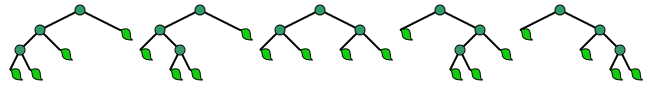
\includegraphics[width=0.7\linewidth]{img/catalan_leaves_binary_tree_example}
		\label{fig:catalanleavesbinarytreeexample}
	\end{figure}
	
	\item $C_n$ es el número de \textbf{caminos monótonos} que se pueden trazar a través de las líneas de una malla de $n \times n$ celdas cuadradas, de forma que nunca se cruce la diagonal. Un camino monótono es aquel que empieza en la esquina inferior izquierda y termina en la esquina superior derecha, y consiste únicamente en tramos que apuntan hacia arriba o hacia la derecha. El recuento de estos caminos es equivalente a contar palabras de Dyck: $X$ significa \emph{moverse a la derecha} e $Y$ significa \emph{moverse hacia arriba}. Los siguientes diagramas muestran el caso n = 3:
	% TODO: \usepackage{graphicx} required
	\begin{figure}[h!]
		\centering
		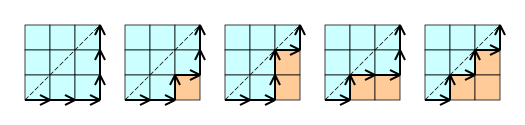
\includegraphics[width=0.7\linewidth]{img/catalan_number_3x3_grid_example}
		\label{fig:catalannumber3x3gridexample}
	\end{figure}
	
	\item $C_n$ es el número de formas distintas de dividir un polígono convexo de $n + 2$ lados en triángulos conectando vértices con diagonales sin que ninguna se corte. La siguiente figura ilustra el caso de las $c_{4} = 14$ posibles triangulaciones para un polígono de $6$ lados:
	% TODO: \usepackage{graphicx} required
	\begin{figure}[h!]
		\centering
		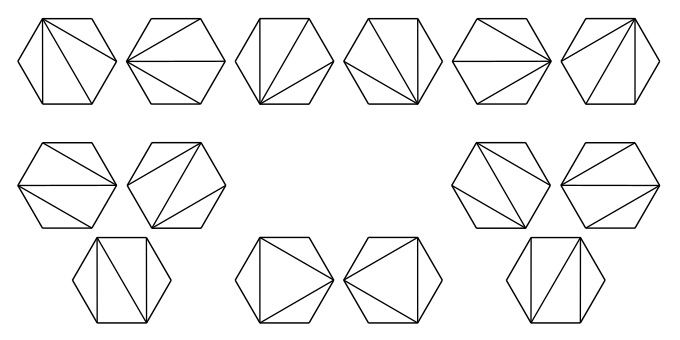
\includegraphics[width=0.7\linewidth]{img/catalan-hexagons-example}
		\label{fig:catalan-hexagons-example}
	\end{figure}

	
	

	
	\item Número de particiones que no se cruzan del conjunto $\{1,\dots, 2n\}$ en el que cada bloque es de tamaño $2$. Una partición no se cruza si y solo si en su diagrama plano, los bloques están disjuntos (es decir, no se cruzan). Por ejemplo, debajo de dos hay particiones cruzadas y no cruzadas de $\{1, 2, 3, 4, 5, 6, 7, 8, 9\}$. La partición $\{\{1, 5, 7\}, \{2, 3, 8\}, \{4, 6\}, \{9\}\}$ se cruza y la partición $\{\{1, 5, 7\}, \{2, 3\}, \{4\}, \{6\}, \{8, 9\}\}$ no se cruza.
	
	% TODO: \usepackage{graphicx} required
	\begin{figure}[!h]
		\centering
		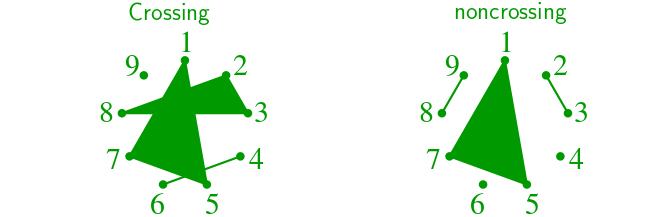
\includegraphics[width=0.7\linewidth]{img/partitiomcopy}
		\label{fig:partitiomcopy}
	\end{figure}
	
	\item Número de permutaciones de longitud $n$ que se pueden ordenar por pila (es decir, se puede demostrar que el reordenamiento se ordena por pila si y solo si no existe tal índice $i < j < k$, tal que $a_k < a_i < a_j$.
	
	\item El número de formas de conectar los puntos $2n$ en un círculo para formar $n$ cuerdas disjuntas.
	
	\item El número de árboles binarios completos no isomorfos con $n$ nodos internos (es decir, nodos que tienen al menos un hijo).
	
	\item El número de formas de cubrir la escalera $1 \ldots n$ usando $n$ rectángulos (la escalera consta de $n$ columnas, donde $i^{th}$ columna tiene una altura $i$). La siguiente figura ilustra el caso n = 4:
	% TODO: \usepackage{graphicx} required
	\begin{figure}[h!]
		\centering
		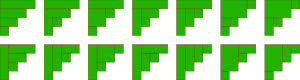
\includegraphics[width=0.7\linewidth]{img/unnamed-2}
		\label{fig:unnamed-2}
	\end{figure}
	
	
	\item Número de formas de formar una cordillera con $n$ tramos ascendentes y $n$ tramos descendentes que se mantienen por encima de la línea original. La interpretación de la cadena montañosa es que las montañas nunca bajarán del horizonte.
	
	\item Puede haber una cantidad de árboles binarios sin etiquetar diferentes con $n$ nodos.
	
	\item Número de permutaciones de $\{1,\dots, n\}$ que evitan el patrón $123$ (o cualquiera de los otros patrones de longitud $3$); es decir, el número de permutaciones sin una subsecuencia creciente de tres términos. Para $n = 3$, estas permutaciones son $132, 213, 231, 312$ y $321$. Para $n = 4$, son $1432, 2143, 2413, 2431, 3142, 3214, 3241, 3412, 3421, 4132, 4213, 4231, 4312$ y $4321$
	
\end{enumerate}